\documentclass[mathserif,9pt]{beamer}
%\usepackage{setspace}
\usepackage[ruled,linesnumbered,vlined]{algorithm2e} % 
\usepackage[utf8]{inputenc}
\usepackage[english]{babel}
\usepackage{caption}
\usepackage{subcaption}
\usepackage{xcolor}
\usepackage{verbatim}
\usepackage{graphicx}
\usepackage{amsmath}
\usepackage{listings}
%\usepackage[round,sort]{natbib}
%\newcommand{\newblock}{} % for natbib
\usepackage{enumerate}
\usepackage[citetracker=true,citestyle=alphabetic, style=verbose,backend=bibtex]{biblatex} 

\usepackage{multirow}
%\usepackage{tikz}

\addbibresource{bib}

\usetikzlibrary{matrix}
\usetikzlibrary{arrows}
\usetikzlibrary{fit}


\renewcommand{\footnotesize}{\tiny}

\numberwithin{figure}{section}
\numberwithin{equation}{section}

\SetAlFnt{\small}
\SetAlCapFnt{\small}


\lstset{ %
  language=C++,                % the language of the code
  basicstyle=\small,  % the size of the fonts that are used for the code
  numbersep=5pt,                  % how far the line-numbers are from the code
  frame=none,                   % adds a frame around the code
  tabsize=2,                      % sets default tabsize to 2 spaces  
  breakatwhitespace=false,        % sets if automatic breaks should only happen at whitespace
  title=\lstname,                   % show the filename of files included
  keywordstyle=\small\color{blue}\bfseries,
  numberstyle=\tiny\color{black},        % line number style
  commentstyle=\tiny\color{teal},       % comment style
  stringstyle=\color{mauve},         % string literal style
  escapeinside={\%*}{*)},            % if you want to add a comment within your code
  aboveskip=0pt,
  belowskip=15pt, 
  abovecaptionskip=0pt, 
  belowcaptionskip=0pt,
  columns=fullflexible%,
  %morekeywords={void,size_t,static_assert,...} % add more keywords
}

\beamertemplatenavigationsymbolsempty
\addtobeamertemplate{footnote}
%\setbeamertemplate{caption}[numbered]



\DeclareGraphicsExtensions{.pdf,.png,.jpg,.jpeg}
%\usecolortheme{beetle}
%\usecolortheme{seagull}
%\usecolortheme{fly}
\usecolortheme{lily}
%\usecolortheme{whale}
\useoutertheme{infolines}

%\usetheme{Madrid}
%\usetheme{Bergen}
\usetheme{Boadilla}
\usefonttheme{serif}
\usefonttheme{structuresmallcapsserif}



\makeatletter
%\setbeamertemplate{frametitle}
%{%
%\vspace{\beamer@headheight}
%
%\begin{beamercolorbox}[wd=\paperwidth,dp=0ex, ht=4ex, sep=0.0ex, colsep*=0pt]{frametitle}%
%\raisebox{-1ex}[0pt][0pt]{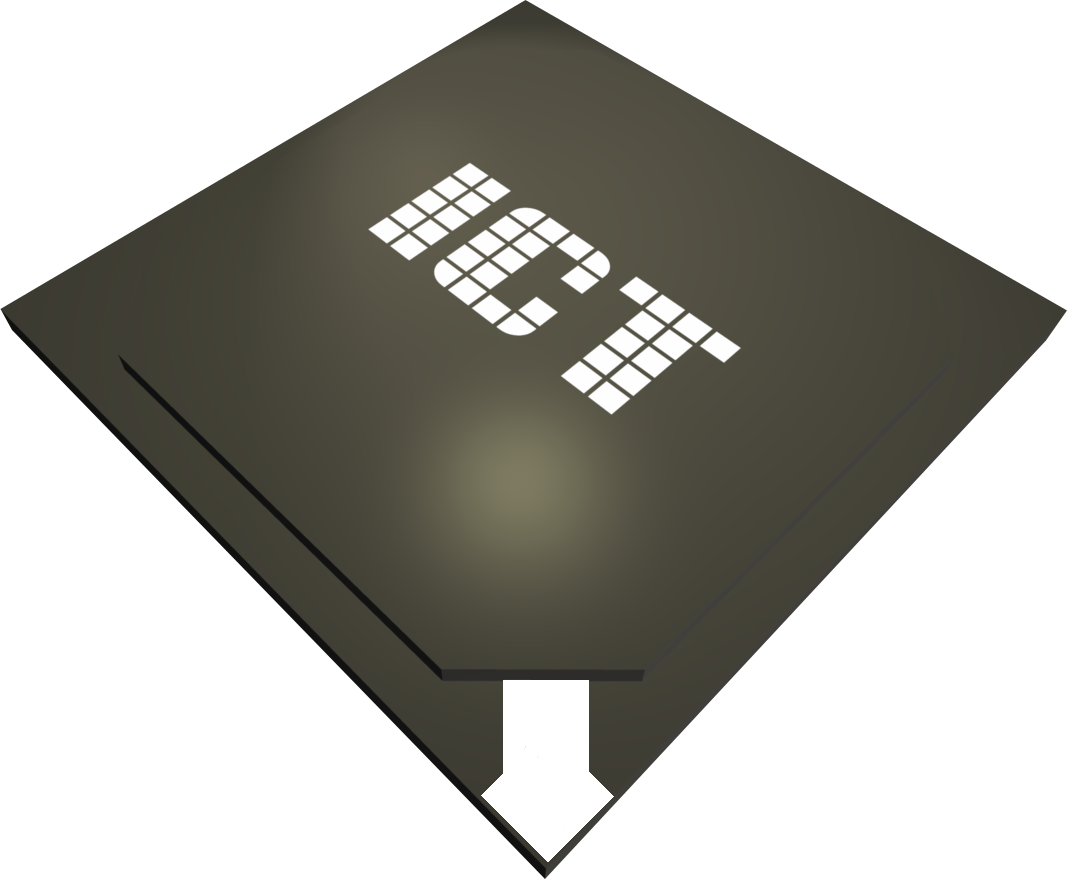
\includegraphics[height=5ex]{figures/ictlogo.png}}%
%\hfill
%\makebox(100,20){
%\usebeamerfont{frametitle}%
%\insertframetitle%  \hfill%\strut 
%}
%\hfill
%\raisebox{1ex}[0pt][0pt]{
\includegraphics[height=2ex]{figures/tuhh.png}}%
%\end{beamercolorbox}%
%}%
\makeatother


%%%%%%%%%%%%%%%%%%%%%%%%%%%%%%%%%%%%%%%%%%%
% Definitions for the presentation
\titlegraphic{
\makebox(200,40){
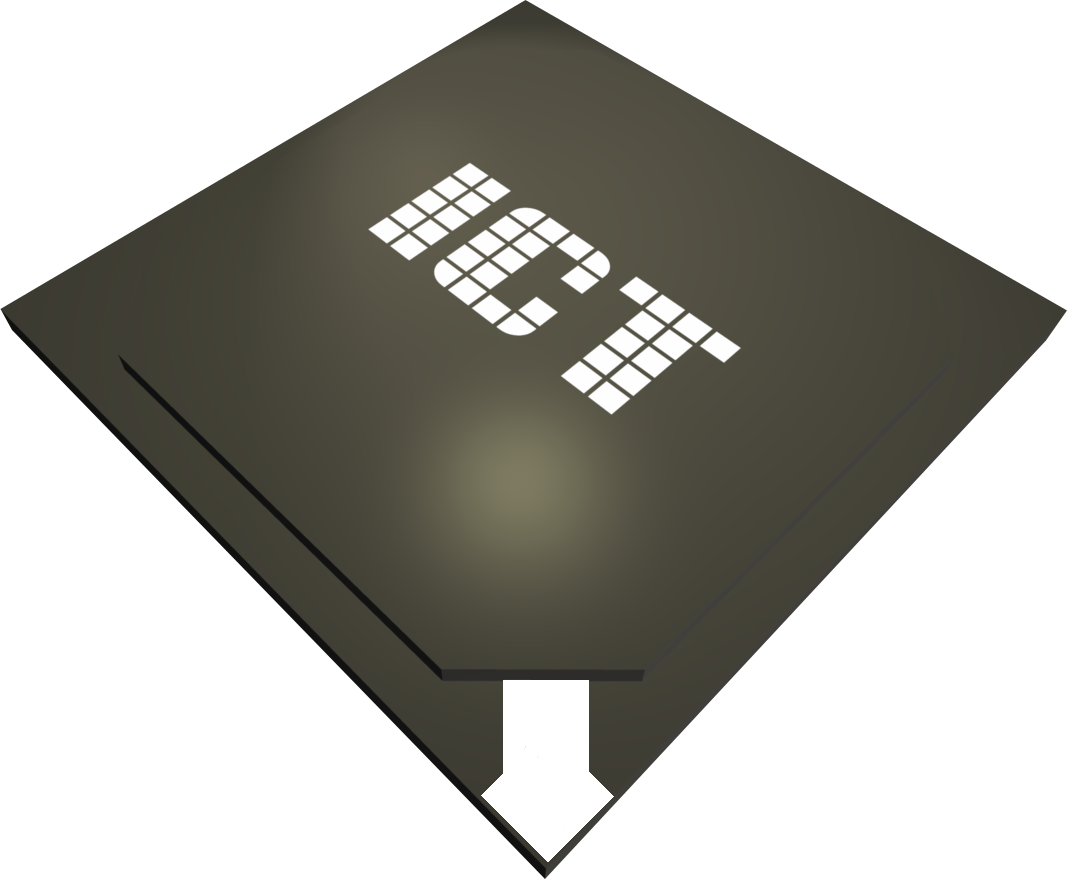
\includegraphics[width=2cm]{figures/ictlogo.png}
}
\makebox(200,40){

\includegraphics[width=4cm]{figures/tuhh.png}
}
}



\title[Untertitel]{Titel}
%\subtitle{}
\author[Autor]{Autor}
\institute[ICT]{Institute of Computer Technology}


%%%%%%%%%%%%%%%%%%%%%%%%%%%%%%%%%%%%%%%%%%%
\makeatletter
\setbeamertemplate{title page}
{
  %\vbox{}
  %\vfill
  \begin{centering}
  \makebox(200,80){{\usebeamercolor[fg]{titlegraphic}\inserttitlegraphic\par}}
    \begin{beamercolorbox}[sep=8pt,center]{title}
      \usebeamerfont{title}\inserttitle
      \vskip0.25em
      {\usebeamerfont{subtitle}\usebeamercolor[fg]{subtitle}\insertsubtitle\par}
    \end{beamercolorbox}
    \vskip1em\par
    \begin{beamercolorbox}[sep=8pt,center]{author}
      \usebeamerfont{author}\insertauthor
    \end{beamercolorbox}
    \vskip-1em\par % change here
    \begin{beamercolorbox}[sep=8pt,center]{institute}
      \usebeamerfont{institute}\insertinstitute
    \end{beamercolorbox}
    \begin{beamercolorbox}[sep=8pt,center]{date}
      \usebeamerfont{date}\insertdate
    \end{beamercolorbox}\vskip0.5em
  \end{centering}
  \vfill
}
\makeatother
%%%%%%%%%%%%%%%%%%%%%%%%%%%%%%%%%%%%%%%%%%%

\begin{document}

\titlepage

% The second page is the table of contents
\frame{
	\frametitle{Overview}
	\tableofcontents%[hidesubsections]
}

\section{Introduction}


\begin{frame}
\frametitle{Lets motivate people!}
\begin{enumerate}
\item What is this all about?
\item Why do I want to present this stuff? 
\item What can people expect from my presentation?
\item (What are the things I did not cover?)
\item (What did other people do?)
\end{enumerate}
\end{frame}


\begin{frame}[fragile]
\frametitle{Greate Example for Motivation}
You can set your own language in folien.tex
\begin{columns}
\begin{column}{0.5\textwidth}
\begin{lstlisting}[basicstyle=\small,keywordstyle=\small\color{blue}]
template <class T>
class CoolClass
{
public:
	CoolClass ();
  CoolClass (const CoolClass&);
  //...
}
\end{lstlisting}
\end{column}
\begin{column}{0.5\textwidth}
\begin{lstlisting}[basicstyle=\small,keywordstyle=\small\color{blue}]
template <class T>
class NextCoolClass
{
public:
	NextCoolClass ();
  NextCoolClass (const NextCoolClass&);
  //...
}
\end{lstlisting}
\end{column}
\end{columns}
\end{frame}


\section{Basic Work}


\subsection{Some of the basic work}

\begin{frame}
\frametitle{Great Frame}
A multidimensional array is a data structure which holds a set of data all of the same type whose elements are arranged in a rectangular pattern\footcite{ISO:2010:Fortran}.
\begin{Definition}[$N$-Way Array]
\label{def:array}
An $n$-way array is really nice!
\end{Definition}
\end{frame}


\begin{frame}
\frametitle{Notation}
Arrangement of the elements of a multidimensional array $\mathbf{A}$ of rank $n$ is given by
\begin{equation}\label{equ:array}
\mathbf{A} = (a_{x_1,\dots,x_n}).
\end{equation}%
Now this is complicated!
\begin{example}[Arrangement]
\label{ex:array}
I like arrays!
\begin{align*}
\mathbf{A} &=
\begin{pmatrix}
a_{0,0,0} & a_{0,1,0} & & a_{0,0,1} & a_{0,1,1} & & a_{0,0,2} & a_{0,1,2} \\
a_{1,0,0} & a_{1,1,0} & & a_{1,0,1} & a_{1,1,1} & & a_{1,0,2} & a_{1,1,2} \\
a_{2,0,0} & a_{2,1,0} & & a_{2,0,1} & a_{2,1,1} & & a_{2,0,2} & a_{2,1,2} \\
a_{3,0,0} & a_{3,1,0} & & a_{3,0,1} & a_{3,1,1} & & a_{3,0,2} & a_{3,1,2}
\end{pmatrix}.
\end{align*}
\end{example}
\end{frame}


\subsection{Other basic work}




\section{Implementation}


%%%%%%%%%%%%%%%%%%%%%%%%%%%%%%%%%%%%
\subsection{Implementation part I}
%%%%%%%%%%%%%%%%%%%%%%%%%%%%%%%%%%%%

\begin{frame}
\frametitle{Important Details!}
Lets be honest, no one can really understand the stuff in detail in 30 minutes as you know!
\begin{itemize}
\item So lets sketch stuff so everyone can understand the details.
\item Point out the really important stuff!
\item Pictures, gestures and everything else might help, but do not exaggerate!
\end{itemize}
\end{frame}


\begin{frame}
\frametitle{Important Results!}
Lets show the people that the implementation is cool! 
But diagrams are generally not drawn well, because:
\begin{itemize}
\item they do not depict the important result! show the important stuff, you want to tell!
\item they do not relate to the implementation!
\item their axis titles cannot be read in most cases. Need big fonts!
\item thir lines are not visible as color and size are not set appropriate.
\item their axis titles are not descriptive and do not have any dimension!
\item their lines are to close! You cannot really distinguish between results!
\end{itemize}
\end{frame}




%\section{Tensor Operations}

\subsection{Elementwise Tensor Operations}
\begin{frame}
\frametitle{}
\begin{Definition}[Elementwise Tensor Operations]
\label{def:elementwise}
Using the notation in Eq. \eqref{equ:array}, an elementwise operation $\boxdot$ is performed by applying a binary operation $\odot$ on the elements of two tensors $\bA$ and $\bB$ of rank $n$ producing a new array $\bC = \bA \boxdot \bB$ with the same shape vector as $\mbd_{A}$ and $\mbd_{B}$, such that
\be\label{equ:elementwise}
\bC[x_1,\dots,x_n] = \bA[x_1,\dots,x_n] \odot \bB[x_1,\dots,x_n],
\ee
with $x_i \in X_i$ for $i = 1,\dots,n$ and $\mbd_{A} = \mbd_{B} = \mbd_{C}$. 
\end{Definition}
\vfill

\emph{Note1: Elements of the data structures must be applicable for the binary operation.}\newline

\emph{Note2: Subtensors may also be used, even for $\bC$ such that $\bC = \bhC$ with $\mbd_{A} = \mbd_{B} = \mathbf{{\hat{d}}}_{C}$.}\newline

\emph{Note3: Eq. \eqref{equ:elementwise} denotes a general form of an elementwise operation which can be specialized with minor changes in order to yield better space and/or time complexity.}
\footcitetext{Bader:2006:Algorithm862}
\end{frame}

\begin{frame}
\frametitle{Notational an algorithm for $\bC = \bA \boxdot \bB$}
\begin{figure}
\begin{minipage}{0.8\textwidth} 
\begin{algorithm}[H]
%\SetAlgoNoLine
\DontPrintSemicolon
\SetKwProg{Fn}{}{}{end}
\SetKwFunction{Map}{Map}%
%\SetAlgoNoEnd
\SetAlgoVlined
\Fn{\Map{$\bC, \bA, \bB, \mbd $}}{
		\For{$x_1 \leftarrow 0$ \KwTo $d_1-1$}
		{
			\For{$x_2 \leftarrow 0$ \KwTo $d_2-1$}
			{
				$\vdots$\;
				\For{$x_n \leftarrow 0$ \KwTo $d_n-1$}
				{
					$\bC(x_1,\dots,x_n) \leftarrow \bA(x_1,\dots,x_n) \odot \bB(x_1,\dots,x_n)$\;
				}				
			}			
		}
}
\caption{$\bC \leftarrow \bA \boxdot \bB$, elementwise operation for $n$-way arrays.\label{alg:map1}}
\end{algorithm}%
\end{minipage}
\end{figure}
\vfill
Characterization:
\bi
\item algorithm consists of $n$ nested loops,
\item $j$ is responsible for iterating over the $j$-th dimension,
\item induction variable $x_j$ is incremented from $k$ to $d_j$,
\item the binary operation $\odot$ is performed in the most inner loop.
\ei

\vfill

\emph{Note: The following algorithms are designed for row-major format, starting at $j=1$ until $j=n$ is reached. The most inner loop will iterate on contiguous elements of arrays.}
\end{frame}

%%%%%%%%%%%%%%%%%%%
%%%%%%%%%%%%%%%%%%%
%%%%%%%%%%%%%%%%%%%

\begin{frame}
\frametitle{Simple Approach (Variant $1$)}
\begin{figure}
\begin{minipage}{0.6\textwidth} 
\begin{algorithm}[H]
%\SetAlgoNoLine
\DontPrintSemicolon
\SetKwProg{Fn}{}{}{end}
\SetKwFunction{Map}{Map1}%
%\SetAlgoNoEnd
\SetAlgoVlined
\tcp{$p' = p - 1$}
\Fn{\Map{$\bC, \bA, \bB, p'$}}{
	\For{$y \leftarrow 0$ \KwTo $p'$}
	{
		$\bC[y] \leftarrow \bA[y] \odot \bB[y]$\;
	}
}
\caption{$\bC \leftarrow \bA \boxdot \bB$.\label{alg:map1}}
\end{algorithm}%
\end{minipage}
\end{figure}
\vfill
\begin{columns}
\begin{column}{.45\textwidth}
Running time (best-case) with arrays:
\be\label{equ:time_map21}
T_{\text{Map2}}(\mbd,n) = (c_2 + c_3)\prod_{i=1}^n d_i = 6\cdot \tau_n,
\ee
where $n-m$ is the number of subscript triplets and $0 \leq m\leq n$ equals the number of tuple subscripts.
\end{column}
%%%%%%%
\begin{column}{.45\textwidth}
%\vskip-3em
Running time (worst-case) with views:
\be\label{equ:time_map2}
\begin{split}
T_{\text{Map1}}(\mathbf{d},n) &= (c_2 + c_3 + 3 \cdot T_h)\cdot \tau_n, \\
                              &= (3\cdot (12n-m+1) + 8) \cdot \tau_n,\\
\end{split}
\ee
with $m \leq n$ which denotes to the number of memory accesses.
\end{column}
\end{columns}
\end{frame}


%%%%%%%%%%%%%%%%%%%
%%%%%%%%%%%%%%%%%%%
%%%%%%%%%%%%%%%%%%%

\begin{frame}
\frametitle{Recursion (Variant $2$)}
\begin{figure}
\begin{minipage}{0.9\textwidth} 
\begin{algorithm}[H]
%\SetAlgoNoLine
\DontPrintSemicolon
\SetKwProg{Fn}{}{}{end} %
\SetKwFunction{Map}{Map2}%
\SetKwFunction{Forward}{Forward}%
%\SetAlgoNoEnd
\SetAlgoVlined
\tcp{\tiny{$n' = n - 1$,  $j$ starts with $0$ and $\mbd_A' = \mbd_A + k$}}
\Fn{\Map{$n', j,\ \ \bC, \bx_C, k_C,\ \  \bA, \bx_A, k_A,\mbd_A',\ \  \bB, \bx_B, k_B$}}
{
	\uIf{$j < n'$ }
	{
		$j' \leftarrow j + 1$\;
		\For(\tcp*[f]{incr $x_B$,$x_C$ by $1$})
		{$x_{A,B,C} \leftarrow k_{A,B,C}$ \KwTo $\mbd_A'[j]$}
		{
			$\bx_{A,B,C}[j] \leftarrow x_{A,B,C}$\;
			\Map{$n', j', \bC, \bx_C, k_C,\ \ \bA, \bx_A, k_A,\mbd_A',\ \ \bB, \bx_B, k_B$}
		}
	}
	\Else
	{
		\For(\tcp*[f]{incr $x_B$,$x_C$ by $1$})
		{$x_{A,B,C} \leftarrow k_{A,B,C}$ \KwTo $\mbd_A'[n']$}
		{
			$\bx_{A,B,C}[n'] \leftarrow x_{A,B,C}$\;
			$\bC(\bx_C) \leftarrow \bA(\bx_A) \odot \bB(\bx_B)$
		}	
	}	
}
\caption{$\bC \leftarrow \bA \boxdot \bB$\label{alg:map2}}
\end{algorithm}%
\end{minipage}
\end{figure}

The running time is given by 
\be
\begin{split}
T_{\text{\ttt{Map2}}} (\mbd,n) %&= c_2\tsum{0}{n-1} + (c_3 + c_4')\tsum{0}{n-2} + (c_4'' + c_5 + c_6) \tsum{1}{n-1} + c_8'\tau_{n-1} + (c_8''+c_9 + c_{10})\tau_n, \\
                               &= \csum{2}{6}\tsum{0}{n-1} + (c_8'' + c_9 + c_{10})\tau_n + (c_{8}'-c_3 - c_4') \tau_{n-1} - \csum{4}{6} , \\
                               &= 30\tsum{0}{n-1} + (q\cdot T_{f\circ g} + q'\cdot T_f + 10)\tau_n - \tau_{n-1} - 24,
\end{split}
\ee
with $0 \leq q \leq 3$, $q' = 3-q$ and $\tau_i = \prod_{j=0}^i d_j$.
\end{frame}


%%%%%%%%%%%%%%%%%%%
%%%%%%%%%%%%%%%%%%%
%%%%%%%%%%%%%%%%%%%

\begin{frame}
\frametitle{Refinement}
\begin{figure}
\begin{minipage}{0.9\textwidth} 
\begin{algorithm}[H]
%\SetAlgoNoLine
\DontPrintSemicolon
\SetKwProg{Fn}{}{}{end} %
\SetKwFunction{Map}{Map3}%
\SetKwFunction{Forward}{Forward}%
%\SetAlgoNoEnd
\SetAlgoVlined
\tcp{\tiny{$n' = n - 1$,  $j$ starts with $0$ and $\mbd_A' = \mbd_A + k$}}
\Fn{\Map{$n', j,\ \ \bC, \bx_C, k_C,\ \  \bA, \bx_A, k_A,\mbd_A',\ \  \bB, \bx_B, k_B$}}
{
	\uIf{$j < n'$ }
	{
		$j' \leftarrow j + 1$\;
		\For(\tcp*[f]{incr $x_B$,$x_C$ by $1$})
		{$x_{A,B,C} \leftarrow k_{A,B,C}$ \KwTo $\mbd_A'[j]$}
		{
			$\bx_{A,B,C}[j] \leftarrow x_{A,B,C}$\;
			\Map{$n', j', \bC, \bx_C, k_C,\ \ \bA, \bx_A, k_A,\mbd_A',\ \ \bB, \bx_B, k_B$}
		}
	}
	\Else
	{
		\For(\tcp*[f]{incr $x_B$,$x_C$ by $1$})
		{$x_{A,B,C} \leftarrow k_{A,B,C}$ \KwTo $\mbd_A'[n']$}
		{
			$\bx_{A,B,C}[n'] \leftarrow x_{A,B,C}$\;
			$\bC(\bx_C) \leftarrow \bA(\bx_A) \odot \bB(\bx_B)$
		}	
	}	
}
\end{algorithm}%
\end{minipage}
\end{figure}
\emph{Observation:} Only the $j$-th element $x_j \in X_j$ of the tuple $\bx$ is modified in the $j$-th call.\newline

\emph{Conclusion:} Split transformation into several index computations. Given zero-based indices $x_i' \in \{0,\dots,d_i-1\}$, $y \in Y$ can be rewritten to
\be\label{equ:map4}
y = \sum_{i=1}^n \mu(x_i',\delta) + k',
\ee
with $\mu_A(x_i',\delta) = x_i'\delta_i$ and $k' = k$ in case of a multidimensional array and $\mu_A(x_i') = g_i(x_i')\delta_i$ and $k' = k\sum_{i=1}^n \delta_i$ in case of view.
\end{frame}


%%%%%%%%%%%%%%%%%%%
%%%%%%%%%%%%%%%%%%%
%%%%%%%%%%%%%%%%%%%

\begin{frame}
\frametitle{Refined Algorithm (Variant $3$)}
\begin{figure}
\begin{minipage}{0.9\textwidth} 
\begin{algorithm}[H]
%\SetAlgoNoLine
\DontPrintSemicolon
\SetKwProg{Fn}{Function}{}{end}
\SetKwFunction{Map}{Map3}%
\SetKw{KwWith}{with}
\SetAlgoVlined
\tcp{$n' = n - 1$ and $j$ starts with $0$}
\Fn{\Map{$n', j,\ \ \bC, y_C,\mbdelta_C,\ \  \bA, y_A,\mbdelta_A,\mbd_A',\ \  \bB,\mbdelta_B, y_B$}}
{
	\uIf{$j < n'$ }{
		$j' \leftarrow j + 1$\;
		\For{$x'\leftarrow 0$ \KwWith $1$ \KwTo $\mbd_A'[n']$}
		{
			$y_{A,B,C} \leftarrow  y_{A,B,C} + \mu(x',\mbdelta_{A,B,C}[j])$\;
			\Map($n', j',\ \  \bC, y_C,\mbdelta_C,\ \  \bA, y_A,\mbdelta_A,\mbd_A',\ \  \bB,\mbdelta_B, y_B$)\;
		}
	}
	\Else
	{
		\For{$x'\leftarrow 0$ \KwWith $1$ \KwTo $\mbd_A'[n']$}
		{
			$y_{A,B,C} \leftarrow  y_{A,B,C} + \mu(x',\mbdelta_{A,B,C}[j])$\;
			$\bC[y_C]$ $\leftarrow$ $\bA[y_A]$ $\odot$ $\bB[y_B]$\;
		}
	}
}
\caption{$\bC \leftarrow \bA \boxdot \bB$\label{alg:map4}}
\end{algorithm}%
\end{minipage}
\end{figure}
The running time corresponds to 
\be\label{equ:time_map3}
\begin{split}
T_{\text{\ttt{Map3}}} (\mbd,n) %&= \csum{2}{6}\tsum{0}{n-1}-(c_8'+c_9'-c_5'-c_4'-c_3')\tau_{n-1} + (c_8'' + c_9'' + c_{10})\tau_n - (c_4''+c_5''+c_6),  \\
                               &= (34+q')\tsum{0}{n-1} + (16+q')\tau_n - \tau_{n-1} - (q'+27),
\end{split}
\ee
with $q'=q_1 + q_2 + q_3$ and $q_i =1$ (array), $q_i=2$ (tuple subscript), $q_i = 3$ (triplet).\newline

\emph{Note: factor multiplied with $\tau_n$ does not contain rank $n$.}
\end{frame}



%%%%%%%%%%%%%%%%%%%
%%%%%%%%%%%%%%%%%%%
%%%%%%%%%%%%%%%%%%%

\begin{frame}
\frametitle{Theoretical Speed-up (1)}
\begin{figure}
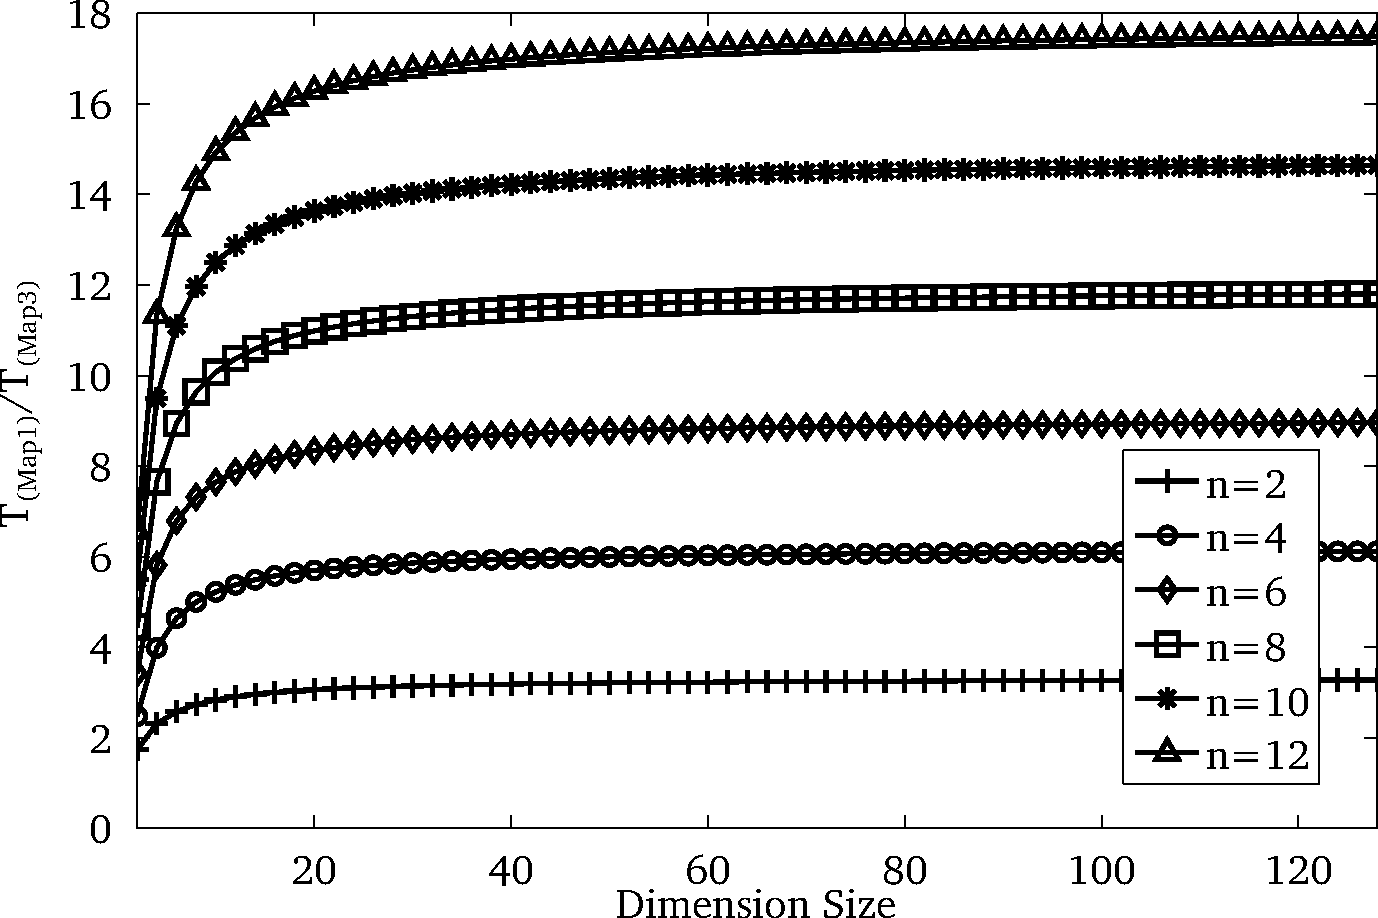
\includegraphics[width=0.7\textwidth]{figures/map13_speedup.pdf}
\caption{Speed-up of $\frac{T_{\text{Map1}}}{T_{\text{Map2}}}$ with $d_i = d$ for all $i\in \{1,\dots,n\}$ in case of views.}
\end{figure}
\end{frame}

%%%%%%%%%%%%%%%%%%%
%%%%%%%%%%%%%%%%%%%
%%%%%%%%%%%%%%%%%%%

\begin{frame}
\frametitle{Theoretical Speed-up (2)}
\begin{table}[tp]%
\label{tab:map}%
\centering %
\begin{tabular}{c|cccc}
              & $\limMap{1}$    & $\limMap{2}$   & $\limMap{3}$    & $\limMap{4}$ \\
\hline\\
Map1    & $1$      & $1.09$       & $1.44n+2.27$  & $3.6n+1.1$ \\
\\
Map2    &  $<1$    & $1$          & $1.32n+1$  & $3.3n+2.5$ \\
\\
Map3    &  $<1$ &  $<1$ & $1$  & $2.5$ \\
\\
Map4    & $<1$ &   $<1$ & $<1$  & $1$ \\
\end{tabular}
\caption{Threshold of speed-ups in case of views.}
\end{table}


Algorithm \ttt{Map4} only uses subscript triplets as range specifiers. In this case we might rewrite the previous equation to
\be
y = \sum_{i=1}^n x_i' \delta_i' + k'
\ee
with $k' = \sum_{i=1}^n (f_i-k) \delta_i + k$ and $\delta_i' = t_i\delta_i$ ($k' = k$ and $t_i = 1$ in case of arrays). Hence, $\delta_i'$ can be used as a stride for each induction variable.
\end{frame}


%%%%%%%%%%%%%%%%%%%
%%%%%%%%%%%%%%%%%%%
%%%%%%%%%%%%%%%%%%%


%%%%%%%%%%%%%%%%%%%%%%%%%%%%%%%%%%%%%%
\subsection{Tensor Multiplication}
%%%%%%%%%%%%%%%%%%%%%%%%%%%%%%%%%%%%%%

\begin{frame}
\frametitle{}
\begin{Definition}[$\bA \times_m \mathbf{u}$]
Let $\bA$ be an tensor with $\mbd_A = (d_1,\dots, d_n)$, $\mathbf{u}$ a vector with $\mbd_U = (\tilde{d}_m, d_m)$, $n\geq 2$ and $1\leq m < n$. The $m$-mode tensor times vector product denoted by $\bA \times_m \mathbf{u}$ returns a new tensor $\bC$ with $\mbd_{\bC} = (d_1,\dots,d_{m-1},d_{m+1}, \dots, d_n)$ which is given by
\be\label{equ:ttv}
\bC(x_1,\dots,x_{m-1},x_{m+1},\dots,x_n) = \sum_{x_m=0}^{d_m-1} \bA(x_1,\dots,x_n) \mathbf{u}(x_m).
\ee
with $\mbd_U[0] = \mbd_A[m-1]$ and $\mbd_C[i] = \mbd_A[i]$ with $i \neq m-1$.
\end{Definition}

\begin{figure}
\centering
\includegraphics[width=0.6\textwidth]{figures/ttv.pdf}
\caption{Example of a $3$-mode tensor-vector multiplication with $\bC = \bA \times_3 \mathbf{u}$}
\label{fig:ttv}
\end{figure}%

\footcitetext{Bader:2006:Algorithm862}
\end{frame}

%%%%%%%%%%%%%%%%%%%
%%%%%%%%%%%%%%%%%%%
%%%%%%%%%%%%%%%%%%%



\begin{frame}
\frametitle{Notational algorithm for $\bA \times_m \mathbf{u}$}
\begin{figure}
\begin{minipage}{0.9\textwidth} 
\begin{algorithm}[H]
%\SetAlgoNoLine
\DontPrintSemicolon
\SetKwProg{Fn}{}{}{end}
\SetKwFunction{TTV}{TTV}%
%\SetAlgoNoEnd
\SetAlgoVlined
\Fn{\TTV{$\bC, \mbd_C, \bA, \mbd_A, \mathbf{u}$}}
{
	\For{$x_1 \leftarrow 0$ \KwTo $d_1-1$ }
	{
		$\vdots$\;
		\For{$x_{m-1} \leftarrow 0$ \KwTo $d_{m-1}-1$ }
		{
			\For{$x_{m+1} \leftarrow 0$ \KwTo $d_{m+1}-1$ }
			{
				$\vdots$\;
				\For{$x_n \leftarrow 0$ \KwTo $d_n-1$ }
				{
					$c = \bC(x_1,\dots,x_{m-1},x_{m+1},\dots,x_{n})$\;
					\For{$x_m \leftarrow 0$ \KwTo $d_m-1$ }
					{
						$c \leftarrow c + \bA(x_1,\dots,x_n) \cdot \mathbf{u}(x_m)$\;
					}
				}
			}
		}
	}
}
\caption{$\bC \leftarrow \bA \times_m \mathbf{u}$\label{alg:ttv}}
\end{algorithm}%
\end{minipage}
\end{figure}
\end{frame}

%%%%%%%%%%%%%%%%%%%
%%%%%%%%%%%%%%%%%%%
%%%%%%%%%%%%%%%%%%%

\begin{frame}
\frametitle{Variant (1)}
\begin{figure}
\begin{minipage}{0.9\textwidth} 
\begin{algorithm}[H]
%\SetAlgoNoLine
\DontPrintSemicolon
\SetKwProg{Fn}{}{}{end}
\SetKwFunction{TTV}{TTV1}%
%\SetAlgoNoEnd
\SetAlgoVlined
\tcp{$m' = m - 1$  and $j,i$ starts with $0$}
\Fn{\TTV{$n, m', j, i,\ \ \bC, k_C, \mbd_C', \bx_C,\ \ \bA, k_A, \mbd_A', \bx_A,\ \ \mathbf{u}, k_u$}}
{
	\uIf{$j = m'$ }
	{
		\TTV{$n,m',j+1, i,\ \ \bC, k_C, \mbd_C', \bx_C,\ \ \bA, k_A, \mbd_A', \bx_A,\ \ \mathbf{u}, k_u$}
	}
	\ElseIf{$j = n$ }
	{
		
		\For(\tcp*[f]{inc $x_C$, $x_u$ by $1$})
		{$x_{A,C,u} \leftarrow k_{A,C,u}$ \KwTo $\mbd_A'[m']$}
		{
			$\bx_{A,C}[m'] \leftarrow x_{A,C}$\;
			$\bC(\bx_C) \leftarrow \bC(\bx_C) + \bA(\bx_A) \cdot \mathbf{u}[x_u]$\;
		}	
	}
	\Else
	{
		$j' \leftarrow j + 1$, $\ i' \leftarrow i + 1$\; 
		\For(\tcp*[f]{inc $x_C$ by $1$})
		{$x_{A,C}\leftarrow k_{A,C}$ \KwTo $\mbd_A'[j]$}
		{
			$\bx_{A}[j] \leftarrow x_{A}$, $\bx_{C}[i] \leftarrow x_{C}$ \;
			\TTV{$j', i',\ \ \bC, k_C, \mbd_C', \bx_C,\ \ \bA, k_A, \mbd_A', \bx_A,\ \ \mathbf{u}, k_u$}\;
		}
	}	
}
\caption{$\bC \leftarrow \bA \times_m \mathbf{u}$\label{alg:ttv1}}
\end{algorithm}%
\end{minipage}
\end{figure}

The running time is given by
\be\label{equ:time_ttv1}
\begin{split}
T_{\text{\ttt{ttv1}}} (\mbd,n) %&= (c_2+c_4+\csum{9}{12})\tsumi{0}{n-1} + (c_5'+c_{10}''+c_{11}+c_{12})\tau_n' + (c_3-4)\tau_{m-1} + \cdots \\ &\qquad\qquad\qquad\qquad + (c_5'' + c_6+c_7)\tau_n - 4\tau_m - (c_{10}''+c_{11}+c_{12}),\\                               
                               &= 35\tsumi{0}{n-1} + 29\tau_{n}' + (13+qT_{f\circ g} + q' T_f)\tau_n - 4\tau_m + 29\tau_{m-1} - 24
\end{split}
\ee
with $q' = 2-q$ and $0\leq q' \leq 2$.
\end{frame}



%%%%%%%%%%%%%%%%%%%
%%%%%%%%%%%%%%%%%%%
%%%%%%%%%%%%%%%%%%%

\begin{frame}
\frametitle{Variant (2)}
\begin{figure}
\begin{minipage}{0.9\textwidth} 
\begin{algorithm}[H]
%\SetAlgoNoLine
\DontPrintSemicolon
\SetKwProg{Fn}{}{}{end}
\SetKwFunction{TTV}{TTV2}%
\SetKw{KwWith}{with}
%\SetAlgoNoEnd
\SetAlgoVlined
\tcp{$m' = m - 1$  and $j,i$ starts with $0$}
\Fn{\TTV{$n,m',j, i,\ \ \bC, \mbdelta_C, y_C,\ \ \bA, \mbdelta_A, \mathbf{e}_A, y_A,\ \ \mathbf{u}$}}
{
	\uIf{$j = m'$ }
	{
		\TTV{$n,m',j+1, i,\ \  \bC, \mbdelta_C, y_C,\ \  \bA, \mbdelta_A, \mathbf{e}_A, y_A,\ \  \mathbf{u}$}
	}
	\ElseIf{$j = n$ }
	{
		$y_u \leftarrow k_u$\;
		\For(\tcp*[f]{incr $y_u$ by $1$ and $y_C$ by $\mbdelta_C[m']$ })
		{$y_{A}$ \KwWith $\mbdelta_A[m']$ \KwTo $\mathbf{e}_A[m']$}
		{
			$\bC[y_C] \leftarrow \bC[y_C] + \bA[y_A] \cdot  \mathbf{u}[y_u]$\;
		}
	}
	\Else
	{
		$j' \leftarrow j + 1$, $\ i' \leftarrow i + 1$\; 
		\For(\tcp*[f]{incr $y_C$ by $\mbdelta_C[i']$})
		{$y_{A}$ \KwWith $\mbdelta_A[j']$ \KwTo $\mathbf{e}_A[j']$}
		{
			\TTV{$n,m',j', i',\ \  \bC, \mbdelta_C, y_C,\ \  \bA, \mbdelta_A, \mathbf{e}_A, y_A,\ \  \mathbf{u}$}
		}		
	}
}
\caption{$\bC \leftarrow \bA \times_m \mathbf{u}$\label{alg:ttv2}}
\end{algorithm}%
\end{minipage}
\end{figure}

The running time is given by
\be\label{equ:time_ttv2}
\begin{split}
T_{\text{\ttt{ttv2}}} (\mbd,n) %&= (c_2+c_4+\csum{9}{11})\tsumi{0}{n-1} + (c_5+c_6'+c_{10}''+c_{11})\tau_n' + (c_3-4)\tau_{m-1} + \cdots \\ &\qquad\qquad\qquad\qquad + (c_6''+c_7)\tau_n - 4\tau_m - (c_{10}''+c_{11}),\\                               
                               &= 38\tsumi{0}{n-1} + 31\tau_{n}' + 11\tau_n - 4\tau_m + 2\tau_{m-1} - 27.
\end{split}
\ee
\end{frame}




\begin{frame}
\frametitle{}
\begin{Definition}[$\bA \times_m \mathbf{u}$]
Let $\bA$ be a tensor with $\mbd_A = (d_1,\dots, d_n)$ and $\mathbf{U}$ a matrix with $\mbd_U = (\tilde{d}_m, d_m)$ and $n\geq 2$ and $1\leq m \leq n$. The $m$-mode product denoted by $\bA \times_m \mathbf{U}$ produces a new tensor $\bC$ with $\mbd_C = (d_1,\dots,d_{m-1},\tilde{d}_m,d_{m+1}, \dots, d_n)$ which is given by
\be\label{equ:mode}
\bC(x_1,\dots,x_{m-1},z_m,x_{m+1},\dots,x_n) = \sum_{x_m=0}^{d_m-1} \mathbf{U}(z_m,x_m) \cdot \bA(x_1,\dots,x_n),
\ee
with $\mbd_U[1] = \mbd_A[m-1]$, $\mbd_U[0] = \mbd_C[m-1]$ and $\mbd_C[i] = \mbd_A[i]$ with $i \neq m-1$.
\end{Definition}

\begin{figure}
\centering
\includegraphics[width=0.6\textwidth]{figures/ttm.pdf}
\caption{Example of a $3$-mode tensor-matrix multiplication with $\bC = \bA \times_3 \mathbf{U}$}
\label{fig:ttm}
\end{figure}%

\footcitetext{Bader:2006:Algorithm862}
\end{frame}

%%%%%%%%%%%%%%%%%%%
%%%%%%%%%%%%%%%%%%%
%%%%%%%%%%%%%%%%%%%



\begin{frame}
\frametitle{Notational algorithm for $\bA \times_m \mathbf{U}$}
\begin{figure}
\begin{minipage}{0.9\textwidth} 
\begin{algorithm}[H]
%\SetAlgoNoLine
\DontPrintSemicolon
\SetKwProg{Fn}{}{}{end}
\SetKwFunction{TTM}{TTM}%
%\SetAlgoNoEnd
\SetAlgoVlined
\Fn{\TTM{$\bC, \mbd_C, \bA, \mbd_A, \mathbf{u}$}}
{
	\For{ $x_1 \leftarrow 0$ \KwTo $d_1-1$ }
	{
		$\vdots$\;
		\For{$x_{m-1} \leftarrow 0$ \KwTo $d_{m-1}-1$ }
		{
			\For{$x_{m+1} \leftarrow 0$ \KwTo $d_{m+1}-1$ }
			{
				$\vdots$\;
				\For{$x_n \leftarrow 0$ \KwTo $d_n-1$ }
				{					
					\For{$z_m \leftarrow 0$ \KwTo $\tilde{d}_m-1$ }
					{
						$c = \bC(x_1,\dots,x_{m-1},z_{m},x_{m+1},\dots,x_{n})$\;
						\For{$x_m \leftarrow 0$ \KwTo $d_m-1$ }
						{
							$c \leftarrow c + \bA(x_1,\dots,x_n) \cdot \mathbf{u}(z_m,x_m)$\;
						}
					}
				}
			}
		}
	}
}
\caption{$\bC \leftarrow \bA \times_m \mathbf{U}$\label{alg:ttm}}
\end{algorithm}%
\end{minipage}
\end{figure}
\end{frame}

%%%%%%%%%%%%%%%%%%%
%%%%%%%%%%%%%%%%%%%
%%%%%%%%%%%%%%%%%%%

\begin{frame}
\frametitle{Variant (1)}
\begin{figure}
\begin{minipage}{0.9\textwidth} 
\begin{algorithm}[H]
%\SetAlgoNoLine
\DontPrintSemicolon
\SetKwProg{Fn}{}{}{end}
\SetKwFunction{TTM}{TTM1}%
%\SetAlgoNoEnd
\SetAlgoVlined
\Fn{\TTM{$n, m', j, i,\ \ \bC, k_C, \mbd_C', \bx_C,\ \ \bA, k_A, \mbd_A', \bx_A,\ \ \mathbf{U}, k_U, \mbd_U',\bx_U$}}
{
	\uIf{$j = m'$ }
	{
		\TTM{$n,m',j+1, i,\ \ \bC, k_C, \mbd_C', \bx_C,\ \ \bA, k_A, \mbd_A', \bx_A,\ \ \mathbf{U}, k_U, \mbd_U',\bx_U$}
	}
	\ElseIf{$j = n$ }
	{	
		$z_U \leftarrow k_U$\;
		\For(\tcp*[f]{incr $z_U$ by $1$})
		{$x_C \leftarrow k_C$ \KwTo $\mbd_C'[m']$}
		{		
			$\bx_C[m'] \leftarrow x_C$, $\bx_U[0] \leftarrow z_U$\;
			\For(\tcp*[f]{incr $x_U$ by $1$})
			{$x_{A,U} \leftarrow k_{A,U}$ \KwTo $\mbd_A'[m']$}
			{
				$\bx_A[m'] \leftarrow x_A$, $\bx_U[0] \leftarrow x_U$\;
				$\bC(\bx_C) \leftarrow \bC(\bx_C) + \bA(\bx_A) \cdot \mathbf{U}(\bx_U)$\;
			}
		}
	}
	\Else
	{
		$j' \leftarrow j + 1$\; 
		\For(\tcp*[f]{incr $x_C$ by $1$})
		{$x_{A,C}\leftarrow k_{A,C}$ \KwTo $\mbd_A'[j]$}
		{
			$\bx_{A,C}[j] \leftarrow x_{A,C}$\;
			\TTM{$j', i',\ \ \bC, k_C, \mbd_C', \bx_C,\ \ \bA, k_A, \mbd_A', \bx_A,\ \ \mathbf{U}, k_U, \mbd_U',\bx_U$}\;
		}
	}
}
\caption{$\bC \leftarrow \bA \times_m \mathbf{U}$\label{alg:ttm1}}
\end{algorithm}%
\end{minipage}
\end{figure}
\be\label{equ:time_ttm1}
\begin{split}
T_{\text{\ttt{ttm1}}} (\mbd,n) %&= (c_2+c_4+\csum{11}{13}) \sum_{\substack{i=0 \\ i \neq m}}^{n-1}\tau_i' + (c_5'+C_{11}+c_{12}')\tau_{n-1}' + c_3\tau_{m-1} + \cdots \\ &\qquad + (c_5'' + \csum{6}{9})\tau_n - (c_5''+ c_6+c_7')\tau_m - (c_{12}''+c_{13}),\\
                               &= 28\left(\sum_{i=0}^{m-1} \tau_m + \frac{1}{d_m}\sum_{i=m+1}^n\tau_i\right)+9\tau_{m-1} - \frac{17\tau_n}{d_m} + \frac{11\tilde{d}_m\tau_n}{d_m} + \dots\\
                               &\qquad\qquad \qquad\qquad\qquad\qquad \dots +  \tilde{d}_m\tau_n(11+qT_{f\circ g} + q'T_f).
\end{split}
\ee
with $0 \leq q \leq 3$, $q' = 3-q$.
\end{frame}



%%%%%%%%%%%%%%%%%%%
%%%%%%%%%%%%%%%%%%%
%%%%%%%%%%%%%%%%%%%

\begin{frame}
\frametitle{Variant (2)}
\begin{figure}
\begin{minipage}{0.9\textwidth} 
\begin{algorithm}[H]
%\SetAlgoNoLine
\DontPrintSemicolon
\SetKwProg{Fn}{}{}{end}
\SetKwFunction{TTM}{TTM2}%
\SetKw{KwWith}{with}
%\SetAlgoNoEnd
\SetAlgoVlined
\tcp{$m' = m - 1$  and $j,i$ starts with $0$}
\Fn{\TTM{$n,m',j, i,\ \ \bC, \mbdelta_C,\mathbf{e}_C, y_C,\ \ \bA, \mbdelta_A, \mathbf{e}_A, y_A,\ \ \mathbf{U}$}}
{
	\uIf{$j = m'$ }
	{
		\TTM{$n,m',j+1, i,\ \  \bC, \mbdelta_C,\mathbf{e}_C, y_C,\ \  \bA, \mbdelta_A, \mathbf{e}_A, y_A,\ \  \mathbf{U}$}
	}
	\ElseIf{$j = n$ }
	{		
		$y_U \leftarrow k_U$\;
		\For(\tcp*[f]{inc $y_U$ by $\mbdelta_U[0]$})
		{$y_C' \leftarrow y_C$ \KwWith $\mbdelta_C[m']$ \KwTo $\mathbf{e}_C[m']$}
		{
			\For(\tcp*[f]{inc $y_U'$ by $\mbdelta_U[1]$})
			{$y_{A,U}'\leftarrow y_{A,U}$ \KwWith $\mbdelta_A[m']$ \KwTo $\mathbf{e}_A[m']$}
			{
				$\bC[y_C'] \leftarrow \bC[y_C'] + \bA[y_A'] \cdot  \mathbf{U}[y_U']$\;
			}
		}
	}
	\Else
	{
		$j' \leftarrow j + 1$\; 		
		\For(\tcp*[f]{inc $y_C$ by $\mbdelta_C[j']$})
		{$y_A$ \KwWith $\mbdelta_A[j']$ \KwTo $\mathbf{e}_A[j']$}
		{
			\TTM{$n,m',j', i',\ \  \bC, \mbdelta_C,\mathbf{e}_C, y_C,\ \  \bA, \mbdelta_A, \mathbf{e}_A, y_A,\ \  \mathbf{U}$}
		}		
	}	
}
\caption{$\bC \leftarrow \bA \times_m \mathbf{U}$\label{alg:ttm2}}
\end{algorithm}%
\end{minipage}
\end{figure}

The running time is given by
\be\label{equ:time_ttm2}
\begin{split}
T_{\text{\ttt{ttm2}}} (\mbd,n) %&= (c_2+c_4+\csum{11}{13}) \sum_{\substack{i=0 \\ i \neq m}}^{n-1}\tau_i' + (c_5'+C_{11}+c_{12}')\tau_{n-1}' + c_3\tau_{m-1} + \cdots \\ &\qquad + (c_5'' + \csum{6}{9})\tau_n - (c_5''+ c_6+c_7')\tau_m - (c_{12}''+c_{13}),\\
                               &= 30\left(\sum_{i=0}^{m-1} \tau_m + \frac{1}{d_m}\sum_{i=m+1}^n\tau_i\right)+9\tau_{m-1} - \tau_n\left(\frac{16}{d_m} + \frac{10\tilde{d}_m}{d_m} +  11\tilde{d}_m\right).
\end{split}
\ee
\end{frame}

\begin{frame}
\frametitle{Speed-up in case of tensor operations}
\begin{table}[tp]%
\label{tab:map}%
\centering %
\begin{tabular}{c|cccc}
          & $\limTTV$   & $\limTTM$   & $\limTTT$  &  $\limMapp$\\
\hline\\
Array    & $2.1n+2.54$  & $2.1n+2.36$ & $3.42n+3.42$ &  $<1$ \\
\\
View     & $3n+2.54$    & $3n+2.36$   & $4.71n+3.42$ & $3.6n+2.5$ \\
\\
\end{tabular}
\caption{Threshold of speed-ups for tensor operations.}
\end{table}

\end{frame}


%\section{Conclusion}

\begin{frame}
\frametitle{Future Work}
\bi
\item Implement tensor operations with \ttt{C++}.
\item Generate empirical results.
\item Compare with other frameworks (measured running time).
\item Extend application area (more operations).
\item Use non-coalesced memory regions for one data structure.
\item Incorporate multi-view spaces (view of a view).
\ei

\centering
\vskip3cm

I should rather stop here!


\end{frame}


%\input{chapters/conc}

\end{document}


